\documentclass[aspectratio=169,compress]{beamer}
\pdfpagewidth\paperwidth
\pdfpageheight\paperheight
\usepackage[italian]{babel}
\usepackage[utf8]{inputenc}
\usepackage[T1]{fontenc}
\usepackage{lmodern,amsmath,amssymb,cclicenses,graphicx,adjustbox,tikz,dsfont,chemfig}
\usetikzlibrary{mindmap}

\DeclareFontFamily{U}{min}{}
\DeclareFontShape{U}{min}{m}{n}{<-> dmjhira}{}
\newcommand{\se}[2]{\ensuremath{\textnormal{\usefont{U}{min}{m}{n}\char"1B}_{#1}^{#2}}}
\newcommand{\1}{\ensuremath{\mathds{1}}}
\newcommand{\Tikz}{Ti\emph{k}Z}

\usetheme[background=light,subsectionpage=progressbar]{metropolis}%numbering=none
\useoutertheme{split}
\hypersetup{pdfstartview={Fit}} % fits the presentation to the window when first displayed

\metroset{block=fill}

\begin{document}
\title{Corso introduttivo a \LaTeX}
\subtitle{Lezione 3}
\author{Davide Peressoni}
\institute[]{Commissione Informatica\\Collegio Universitario don Nicola Mazza}
\date%[DATE CURTE]
{19 Dicembre 2018}
\titlegraphic{
\includegraphics[height=80px]{ComInfo}}

\setbeamertemplate{title page}{
  \begin{minipage}[b][\paperheight]{\textwidth}
    \vfill%
    \ifx\inserttitle\@empty\else\usebeamertemplate*{title}\fi
    \ifx\insertsubtitle\@empty\else\usebeamertemplate*{subtitle}\fi
    \usebeamertemplate*{title separator}
    \vspace*{1cm}
    \adjustbox{valign=M}{\ifx\inserttitlegraphic\@empty\else\usebeamertemplate*{title graphic}\fi}
    \adjustbox{valign=M}{\begin{minipage}{200px}
      \ifx\beamer@shortauthor\@empty\else\usebeamertemplate*{author}\fi
      \ifx\insertdate\@empty\else\usebeamertemplate*{date}\fi
      \ifx\insertinstitute\@empty\else\usebeamertemplate*{institute}\fi
    \end{minipage}}
    \vfill
    \vspace*{1mm}
  \end{minipage}
}
\setbeamertemplate{title graphic}{\inserttitlegraphic}

\maketitle

% \frame{\transfade
%   \frametitle{Table of Contents}
%   \tableofcontents[hideallsubsections]
% }
\frame{
  \tiny\cc 2018 Davide Peressoni\\~\par
    \emph{Le informazioni contenute nel presente docuemnto sono state verificate e documentate con la massima cura possibile. Nessuna responsabilità derivante dal loro utilizzo potrà venire imputata all’Autore coinvolto nella loro creazione, pubblicazione e distribuzione.}\\~\par
    Alcuni diritti riservati.\\~\\
    Documento prodotto con \LaTeX.\\
    Questo documento è rilasciato con licenza\\
    \begin{figure}[!ht]
	\centering
	    
\includegraphics{../Lezione1/CC.pdf}
    \end{figure}~\\
    \textbf{Creative Commons BY-NC-SA 4.0}\\
    Attribuzione – Non Commerciale - Stessa licenza\\
    \url{http://creativecommons.org/licenses/by-nc-sa/4.0/}\\
    \textbf{Attribuzione} — Devi riconoscere una menzione di paternità adeguata, fornire un link alla licenza e indicare se sono state effettuate delle modifiche. Puoi
    fare ciò in qualsiasi maniera ragionevole possibile, ma non con modalità tali da suggerire che il licenziante avalli te o il tuo utilizzo del materiale.\\
    \textbf{Non commerciale} — Non puoi usare il materiale per scopi commerciali.\\
    \textbf{Stessa licenza} — Se remixi, trasformi il materiale o ti basi su di esso, devi distribuire i tuoi contributi con la stessa licenza del materiale originario.
}

\section{Presentazioni}
\begin{frame}\centering
  \frametitle{La classe Beamer}
  \texttt{\textbackslash{}documentclass[aspectratio=169]\{beamer\} \% prima riga} 
  \pause
  \texttt{\\\dots\\
  \textbackslash{}begin\{frame\} \%dentro il document
\\
  ~~\textbackslash{}frametitle\{Titolo\}~~~~~~~~~~~~~
\\
  ~~\textbackslash{}framesubtitle\{Sottotitolo\}~~~~~
\\
  \textbackslash{}end\{frame\}
~~~~~~~~~~~~~~~~~~~~~~~\\~}
\end{frame}
\begin{frame}\centering
  \frametitle{Comandi noti}
  Preambolo: codifica dei caratteri, pacchetti da includere, \dots\\~\\\pause
  Titolo: \texttt{\textbackslash{}maketitle}\\~\\\pause
  \texttt{\textbackslash{}section, \textbackslash{}subsection}\\~\\\pause
  Formattazione testo, immagini, note a piè di pagina, bibliografia, \dots
\end{frame}
\begin{frame}\centering
  \frametitle{Indice}
  \texttt{~\\
  \textbackslash{}begin\{frame\}~~~~~~~~~~~\\
  ~~\textbackslash{}frametitle\{Contenuti\}\\
  ~~\textbackslash{}tableofcontents~~~~~~~~\\
  \textbackslash{}end\{frame\}~~~~~~~~~~~~~\\~
}
\end{frame}
\begin{frame}\centering
  \frametitle{Animazioni}
  \texttt{Questa è \textbackslash{}pause una prova}\\~\\\pause
  Questa è \pause una prova
\end{frame}
\begin{frame}\centering
\frametitle{Temi e colori}
  \begin{tabular}{ll}
    \texttt{\textbackslash{}usetheme\{Warsaw\}}&\only<2->{Esempi di tutte le combinazioni tema-colore: }\\
    \texttt{\textbackslash{}usecolortheme\{seahorse\}} & \only<2->{\url{https://hartwork.org/beamer-theme-matrix/}}
  \end{tabular}
  \visible<2->{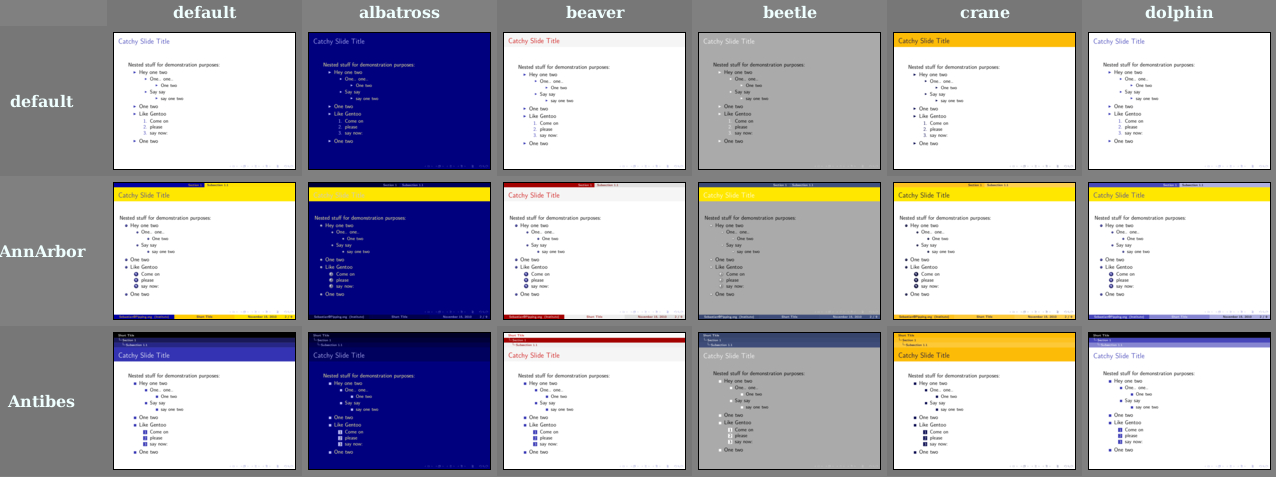
\includegraphics[width=400px]{img/beamer_beamer}}
\end{frame}

\section{\Tikz}
\begin{frame}\centering
\frametitle{\Tikz}
  Libreria grafica per disegnare (descrivere disegni) con LaTeX.\\\pause
  Offre un piano cartesiano su cui disegnare mediante dei comandi.\\~\\\pause
  \texttt{\textbackslash{}usepackage\{tikz\} \%preambolo}\\\pause
  \dots\\\texttt{
  \textbackslash{}begin\{tikzpicture\}\\
  \dots\\
  \textbackslash{}end\{tikzpicture\}~~\\~}
\end{frame}
\begin{frame}\centering
\frametitle{Punti}
  \texttt{(1cm,2pt)} è un punto a coordinata x 1cm dall'origne e y 2pt dall'origine\\~\\\pause
  \texttt{(30:1cm)} è un punto sulla circonferenza di raggio 1 cm, a 30 gradi (coordinate polari)\\~\\\pause
  \texttt{++(1cm,2cm)} le coordinate sono relative a quelle del punto precedente e non all'origine\\~\\\pause
  \texttt{+(1cm,2cm)} come \texttt{++} ma non aggiorna le coordinate dell'ultimo punto
\end{frame}
\begin{frame}\centering
\frametitle{Disegnare}
  \texttt{\textbackslash{}path[opzioni] punti;}\\\pause
  \begin{description}
    \item<2->[path type] \texttt{\textbackslash{}draw}, \texttt{\textbackslash{}fill}, \texttt{\textbackslash{}filldraw}
    \item<3->[geometria] \texttt{rotate=<angolo>}, \texttt{xshift=<length>}, \texttt{yshift}, \texttt{scale=<fattore>}
    \item<4->[colore] \texttt{color=<colore>}, \texttt{draw=<colore>}, \texttt{fill=<colore>}, \texttt{opacity=<fattore>}
    \item<5->[spessore linee] ultra thin, very thin, thin, semithick, thick, very thick, ultra thick
    \item<6->[tratteggio] solid, dashed, dotted, dashdotted, densely dotted, loosely dotted, "double
  \end{description}
\end{frame}
\begin{frame}\centering
\frametitle{Esempi}
  \begin{tabular}{l|l}
    \texttt{\small\textbackslash{}draw (1,0) -\hspace{0.01mm}- (0,0) -\hspace{0.01mm}- (0,1);} & \begin{tikzpicture}\draw (1,0) -- (0,0) -- (0,1);\end{tikzpicture}\\\hline~&~\\
    \texttt{\small\textbackslash{}draw[red, dashed, very thick, rotate=30] (1,0) -\hspace{0.01mm}- (0,0) -\hspace{0.01mm}- (0,1);} & \begin{tikzpicture}\draw[red, dashed, very thick, rotate=30] (1,0) -- (0,0) -- (0,1);\end{tikzpicture} \\\hline~&~\\
    \texttt{\small\textbackslash{}fill (1,0) -\hspace{0.01mm}- (0,0) -\hspace{0.01mm}- (0,1) -\hspace{0.01mm}- cycle;} & \begin{tikzpicture}\fill (1,0) -- (0,0) -- (0,1) -- cycle;\end{tikzpicture}\\\hline~&~\\
    \texttt{\small\textbackslash{}draw (0,0) -| (0.5,1) (1,0) |- (2,1);} & \begin{tikzpicture}\draw (0,0) -| (0.5,1) (1,0) |- (2,1);\end{tikzpicture}
  \end{tabular}
\end{frame}

\subsection{Disegnare}
\begin{frame}\centering
\frametitle{Figure geometriche}
  \begin{tabular}{l|l}
    \texttt{\small\textbackslash{}draw (0,0) rectangle (2,1);} & \begin{tikzpicture}\draw (0,0) rectangle (2,1);\end{tikzpicture}\\\hline~&~\\
    \texttt{\small\textbackslash{}draw (0,0) circle [radius=1];} & \begin{tikzpicture}\draw (0,0) circle [radius=1];\end{tikzpicture} \\\hline~&~\\
    \texttt{\small\textbackslash{}draw  (0,0) circle [x radius=1cm, y radius=5mm, rotate=30];} & \begin{tikzpicture}\draw  (0,0) circle [x radius=1cm, y radius=5mm, rotate=30];\end{tikzpicture}\\
  \end{tabular}
\end{frame}
\begin{frame}\centering
\frametitle{Nodi}
  \begin{tabular}{l|l}\texttt{\small\textbackslash{}draw (0,0) node \{centro\} circle [radius=1];} & \begin{tikzpicture}\draw (0,0) node {centro} circle [radius=1];\end{tikzpicture} \\\hline\\
    \begin{tabular}{l}\texttt{\small\textbackslash{}draw (0,0) node (centro) \{O\} circle [radius=5mm];}\\\texttt{\small\textbackslash{}draw (centro) rectangle ++(1,1);}\end{tabular} & \begin{tikzpicture}\draw  (0,0) node (centro) {O} circle [radius=5mm];\draw (centro) rectangle ++(1,1);\end{tikzpicture}\\
  \end{tabular}
\end{frame}

\subsection{Grafici}
\begin{frame}\centering
  {\tiny\[g(x)=e^x;~~h(x)=x^2;~~i(x)=x-3; ~~f(x)=\begin{cases}  g(x) & x<-1\\
                        h(x) & -1<x<2\\
                        i(x) & x>2
          \end{cases}\]}
  {\centering
    \begin{tikzpicture}[scale=0.7]
      \draw[->] (-9,0) -- (9,0) node[below] {$x$};
      \draw[->] (0,-1.3) -- (0,4.2) node[left] {$y$};
      \draw[loosely dotted] (-8.9,-1.2) grid (8.9,4.2);
      %1-s(x+1)
      \draw[domain=-1:8.9,thick,red] plot ({\x},{0});
      \draw[domain=-9:-1,smooth,red] plot ({\x},{1});
      %s(x+1)[1-s(x-2)]
      \draw[domain=2:8.9,smooth,dashed,green] plot ({\x},{0});
      \draw[domain=-9:-1,smooth,green] plot ({\x},{0});
      \draw[domain=-1:2,smooth,green] plot ({\x},{1});
      %s(x-2)
      \draw[domain=-9:2,smooth,dashed,cyan] plot ({\x},{0});
      \draw[domain=2:9,smooth,cyan] plot ({\x},{1});
      %f(x)
      \draw[domain=-9:-1,smooth,blue] plot ({\x},{e^\x});
      \draw[domain=-1:2,smooth,blue] plot ({\x},{\x*\x});
      \draw[domain=2:7,smooth,blue] plot ({\x},{\x-3});
      \draw[smooth,blue,fill=white] (-1,1/e) circle (1.5pt);
      \draw[smooth,black,fill=white] (-1,1) circle (1.5pt);
      \draw[smooth,blue,fill=white] (2,4) circle (1.5pt);
      \draw[smooth,blue,fill=white] (2,-1) circle (1.5pt);
      \draw[smooth,black,fill=white] (-1,0) circle (1.5pt);
      \draw[smooth,black,fill=white] (2,0) circle (1.5pt);
      \draw[smooth,black,fill=white] (2,1) circle (1.5pt);
    \end{tikzpicture}\par
  }
  {\tiny\[\color{blue}y=f(x)=\frac{1}{2}[e^x+(x+1)^{l-1}(x^2-e^x)-(x-2)^{l-1}(x^2-x+3)+x-3]\]
  \[{\color{red}y=\se{-\infty}{-1}(x)=\1(-x-1)}~~{\color{green}y=\se{-1}{2}(x)}~~{\color{cyan}y=\se{2}{\infty}(x)=\1(x-2)}\]}
\end{frame}
\begin{frame}\centering
  \frametitle{Grafici con \Tikz}
  \begin{flushleft}
    \texttt{~\\
    \textbackslash{}begin\{tikzpicture\}\\
    ~~\%assi cartesiani\\
    ~~\textbackslash{}draw[-\textgreater{}] (-9,0) -\hspace{0.01mm}- (9,0) node[below] \{\textdollar{}x\textdollar{}\};
\\
    ~~\textbackslash{}draw[-\textgreater{}] (0,-1.3) -\hspace{0.01mm}- (0,4.2) node[left] \{\textdollar{}y\textdollar{}\};\\
    ~~\%griglia\\
    ~~\textbackslash{}draw[loosely dotted] (-8.9,-1.2) grid (8.9,4.2);\\
    ~~\%funzione
\\
    ~~\textbackslash{}draw[domain=-1:8.9,thick,red] plot (\{\textbackslash{}x\},\{\textbackslash{}x\^{}2\});
\\
    \textbackslash{}end\{tikzpicture\}\\~
    }
    \end{flushleft}
\end{frame}
\begin{frame}\centering
  \frametitle{Funzioni}
 factorial(x), sqrt(x), pow(x,y), exp(x), ln(x), log10(x), log2(x), abs(x), mod(x,y), round(x), floor(x), ceil(x), sin(x), cos(x), tan(x), min(x,y,) e max(x,y).\\~\\\pause
 Gli argomenti delle funzioni trigonometriche vanno espressi in gradi; per esprimerli in radianti bisogna postporre una \emph{r}.\\~\\\pause
 Si possono usare le costanti: \texttt{e} e \texttt{pi}. 
\end{frame}

\subsection{Mappe Concettuali}
\begin{frame}\centering
  \frametitle{Mindmap}
  \texttt{\textbackslash{}usetikzlibrary\{mindmap\}}
  \hspace*{-1cm}
    \begin{tabular}{cc}
      \begin{tabular}{l}
        \texttt{\tiny\textbackslash{}begin\{tikzpicture\}[mindmap, concept color=yellow]
}\\
        \texttt{\tiny~~\textbackslash{}node [concept] \{Parola chiave\}
}\\
        \texttt{\tiny~~~~child[grow=0] \{}
\\
        \texttt{\tiny~~~~~~node[concept] \{figlio 1\}}
\\
        \texttt{\tiny~~~~~~child[concept color=green] \{node[concept] (nipote) \{nipote\}\}}
\\
        \texttt{\tiny~~~~\}}
\\
        \texttt{\tiny~~~~child[concept color=orange,grow=30] \{node[concept] (figlio) \{figlio 2\}\};}
\\
        \texttt{\tiny~~\textbackslash{}draw [concept connection]  (figlio) edge (nipote);
}\\
        \texttt{\tiny\textbackslash{}end\{tikzpicture\}}
      \end{tabular}
      &
      \begin{tikzpicture}[mindmap, concept color=yellow,scale=0.5,every node/.style={scale=0.5}]
        \node [concept] {Parola\\chiave}
          child[grow=0] {
            node[concept] {figlio 1}
            child[concept color=green] {node[concept] (nipote) {nipote}}
          }
          child[concept color=orange,grow=30] {node[concept] (figlio) {figlio 2}};
          \draw [concept connection]  (figlio) edge (nipote);
      \end{tikzpicture}
    \end{tabular}
\end{frame}

\section{Chimica}
\begin{frame}\centering
  \frametitle{Chemfig}
  \texttt{\textbackslash{}usepackage\{chemfig\} \%preambolo}\\
 \texttt{\textbackslash{}chemfig\{<\textrm{atomo1}><\textrm{bond type}>[<\textrm{angolo}>, <\textrm{lunghezza}>, <\textrm{opzioni \Tikz}>]<\textrm{atomo2}>\}}\\~\\\pause{}Esempi minimali:\\
 \begin{tabular}{l|l}
  \textbackslash{}chemfig\{A-B\}&\chemfig{A-B}\\
\hline
  \textbackslash{}chemfig\{A=B\}&\chemfig{A=B}\\
\hline
  \textbackslash{}chemfig\{A\textasciitilde{}B\}&\chemfig{A~B}\\
\hline
  \textbackslash{}chemfig\{A>B\}&\chemfig{A>B}\\
\hline
  \textbackslash{}chemfig\{A<:B\}&\chemfig{A<:B}\\
\hline
  \textbackslash{}chemfig\{A>|B\}&\chemfig{A>|B}\\
\hline
 \end{tabular}
\end{frame}
\begin{frame}\centering
  \frametitle{Una molecola}
  \texttt{\textbackslash{}chemfig\{C(-[:0]H)(-[:90]H)(-[:180]H)(-[:270]H)\}}\\~\\
  \chemfig{C(-[:0]H)(-[:90]H)(-[:180]H)(-[:270]H)}
\end{frame}
\begin{frame}\centering
  \frametitle{Anelli}
  \texttt{\textbackslash{}chemfig\{A*6(-B-C-D-E-F-)\}}\\~\\
  \chemfig{A*6(-B-C-D-E-F-)}
\end{frame}
\begin{frame}\centering
  \frametitle{Reazioni chimiche}
  \begin{tabular}{l|l}
  \textbackslash{}schemestart A\textbackslash{}arrow\{->\}B\textbackslash{}schemestop&\schemestart A\arrow{->}B\schemestop\\\hline
  \textbackslash{}schemestart A\textbackslash{}arrow\{-/>\}B\textbackslash{}schemestop&\schemestart A\arrow{-/>}B \schemestop\\\hline
  \textbackslash{}schemestart A\textbackslash{}arrow\{<-\}B\textbackslash{}schemestop&\schemestart A\arrow{<-}B \schemestop\\\hline
  \textbackslash{}schemestart A\textbackslash{}arrow\{<->\}B\textbackslash{}schemestop&\schemestart A\arrow{<->}B \schemestop\\\hline
  \textbackslash{}schemestart A\textbackslash{}arrow\{<=>\}B \textbackslash{}+ C\textbackslash{}schemestop&\schemestart A \arrow{<=>}B \+ C\schemestop\\
 \end{tabular}
\end{frame}


\setbeamercolor{background canvas}{bg=black}
\frame[plain]{\transfade}
\end{document}
